%% Based on a TeXnicCenter-Template by Gyorgy SZEIDL.
%%%%%%%%%%%%%%%%%%%%%%%%%%%%%%%%%%%%%%%%%%%%%%%%%%%%%%%%%%%%%

%----------------------------------------------------------
%
\documentclass[a4paper,12pt,reqno]{book}%
%
%----------------------------------------------------------
% This is a sample document for the AMS LaTeX Book or Monograph Class
% Class options
%       --  Body text point size:
%                        8pt, 9pt, 10pt (default), 11pt, 12pt
%       --  Paper size:  letterpaper (8.5x11 inch, default), a4paper
%       --  Orientation: portrait(default), landscape
%       --  Print side:  oneside, twoside (default)
%       --  Quality:     final(default), draft
%       --  Title page:  titlepage, notitlepage
%       --  Start chapter on left:
%                        openright (no, default), openany
%       --  Columns:     onecolumn (default), twocolumn
%       --  Omit extra math features:
%                        nomath
%       --  AMS fonts (noamasfonts available):
%                        noamsfonts
%       --  PSAMSfonts (fewer AMSfontsizes)
%                        psamsfonts
%       --  Equation numbering (equation numbers on the left is the default)
%                        leqno (default), reqno
%       --  Equation centering (equations centered is the default)
%                        centeredtags (default}, tbtags (top, bottom)
%       --  Displayed equations (centered is the default)
%                        fleqn (flush left)
% For instance the command
%          \documentclass[a4paper,12p,reqno]{amsbook}
% ensures that the paper size is a4, fonts are typeset at the size 12p
% and the equation numbers are on the right side.
\usepackage{lscape}
\usepackage{amsmath}%
\usepackage{amsfonts}%
\usepackage{amssymb}%
\usepackage{graphicx}%
\usepackage{chngcntr}%
\usepackage{epsfig}%
\usepackage{multirow}%
\usepackage{longtable}%
\usepackage[utf8]{inputenc}
\usepackage[OT4]{polski}
\usepackage[dvips]{color}%
%\usepackage[left=35mm, right=20mm, top=20mm, bottom=30mm]{geometry}%
\usepackage{geometry}%
\usepackage[titletoc]{appendix}%
\usepackage{raport}%
\usepackage{setspace}%d
 \usepackage{url}%
%----------------------------------------------------------
\onehalfspacing
\numberwithin{equation}{chapter}%
\counterwithout{figure}{section}%
\counterwithout{figure}{chapter}%
%\counterwithout{table}{section}%
%\counterwithout{table}{chapter}%
%-----------------------------------------------------------

%-----------------------------------------------------------
\title{Analiza strumieniowa w internecie rzeczy}
\newcommand{\ownYear}{2016/2017}
\author{Dominik Waśniowski}
\newcommand{\supervisor}{Dr inż. Janusz Granat}
\newcommand{\lcol}[1]{\multicolumn{1}{l}{#1}}
\newcommand{\lcolDash}[1]{\multicolumn{1}{l|}{#1}}
\newcommand{\ccol}[1]{\multicolumn{1}{c}{#1}}
\newcommand{\comma}{\mbox{,}}
%----------------------------------------------------------

\newcommand{\streszczenie}{Abstract}

\newcommand{\streszczenieen}{\textbf{Tile}: English title.\\[3mm]
English abstract
}

\newcommand{\slowakluczowe}{analiza strumieniowa, internet rzeczy, IoT}
\newcommand{\slowakluczoween}{stream analisys, internet of things, IoT}

%-----------------------------------------------------------
\begin{document}
\frontmatter
\newgeometry{centering}
\frontpage
\restoregeometry
\makeabstracts
\tableofcontents
\mainmatter
\chapter{Wprowadzenie}
Szacuje się,
że obecnie w użyciu jest 2 mld komputerów,
10 mld telefonów komórkowych,
a do 2020 r. do sieci ma być podłączone 20 mld urządzeń (Gartner, Inc., 2015).
Urządzenia te będą zbierać dane,
przetwarzać je
bądź przekazywać dalej.
Dzięki temu ludzie będą mogli wiedzieć więcej na temat otaczającego świata,
szybciej reagować na zmiany
czy podejmować lepsze decyzje.
Ogromne ilości danych generowane w każdej sekundzie,
oraz wymagania użytkowników aby wyniki otrzymywać coraz szybciej,
najlepiej od razu,
powodują,
że obecne metody przetwarzania danych stają się niewystarczające.
Wśród rozwiązań pozwalających radzić sobie w takich sytuacjach
coraz większą popularność zyskuje przetwarzanie strumieniowe (\textit{stream analysis, data streaming}).

Rozwiązania oparte na przetwarzaniu strumieniowym charakteryzują się wysoką przepustowością,
krótkimi czasami odpowiedzi i odpornością na awarie.
Dane mogą pochodzić z różnych źródeł: czujniki, komputery, telefony.
Możliwe jest tworzenie i wykonywanie analiz w czasie rzeczywistym,
dane przetwarzane są na bieżąco,
bezpośrednio po ich otrzymaniu.

Jednym z zagadnień związanych z przetwarzaniem danych jest wykrywanie zmian (sytuacji nietypowych).
Przez lata powstało wiele prac starających się rozwiązać ten problem.
Większość z nich oparta jest na analizie całościowej,
tj. zestawy danych,
które poddane są analizie,
przygotowywane są wcześniej i nie ulegają zmianie w czasie.
Algorytmy nie są w stanie na bieżąco analizować napływających danych.

Tematem niniejszej pracy jest zagadnienie wykrywania zmian w przebiegach czasowych,
oparte na mechanizmach statystycznych.

Celem pracy jest stworzenie mechanizmów wykrywających sytuacje nietypowe
z wykorzystaniem technik analizy strumieniowej.
W ramach pracy zostały sprawdzone dostępne platformy streamingowe:
\begin{itemize}
  \item Esper,
  \item Apache Spark,
  \item Apache Storm
\end{itemize}
pod kątem przydatności.
Aby sprawdzić skuteczność analizy strumieniowej zostały zaimplementowane algorytmy Bayesa (\textit{Bayesian Online Changepoint Detection})
oraz ADWIN.
Algorytmy w ramach pracy zostały zaadaptowane do wersji strumieniowych oraz przygotowane pod kątem platformy Apache Storm.
Analiza skuteczności badanych algorytmów została przeprowadzona z wykorzystaniem danych wygenerowanych losowo jak i rzeczywistych.

Układ pracy jest następujący.
Rozdział drugi przybliża tematykę związaną z analizą strumieniową.
W tym samym rozdziale znajduję się także porównanie dostępnych platform.
W rozdziale trzecim przedstawiono teoretyczne aspekty związane z wykrywaniem zmian.
Rozdział czwarty z kolei dokładnie przedstawia wykorzystane algorytmy.
W rozdziale piątym znajdują się wyniki przeprowadzonych eksperymentów.
Ostatni rozdział stanowi podsumowanie.
W dodatku A znajduje spis zawartości płyty CD.


\chapter{Analiza strumieniowa}
\label{ch:tech}
\section{Przetwarzanie danych}
\subsection{Big Data}
Lawinowo rosnąca liczba nowych urządzeń podłączanych do sieci
oraz wzrost tempa generowania danych przez nie spowodowało,
że konieczne się stało stworzenie nowych metod ich analizy.
Klasyczne metody polegające na tworzeniu coraz większych,
mocniejszych komputerów (\textit{vertical scaling})
mierzących się z problemami analizy danych stawały się nie wystarczające.
Głównie ze względów ekonomicznych.
Takie rozwiązania były bardzo kosztowne w utrzymaniu i szybko stawały się przestarzałe.
Trzeba było szukać pomysłów w innym miejscu.
Zaczęto łączyć mniejsze komputery razem (\textit{horizonal scaling}),
by mogły rozwiązywać większe problemy.
Pojawiły się pierwsze rozwiązania gridowe,
obliczenia chmurowe (\textit{cloud computing})
czy mechanizmy typu \textit{MapReduce}.
Tematykę oraz wszystko co było w okół niej,
związana z masową analizą danych nazwano \textit{Big Data}.

Dane \textit{Big Data} można w skrócie opisać modelem \textit{3V} (Gartner Inc., 2012):
\begin{itemize}
		\item \textbf{Volume} - ilość,
		której nie można przetworzyć z wykorzystaniem standardowych metod i narzędzi.
		\item \textbf{Velocity} - zmienność.
		Dane napływają z różną częstotliwością (natężeniem),
		często w tym samym momencie.
		\item \textbf{Variety} - różnorodność.
		Dane pochodzą pochodzą z wielu źródeł.
		Mogą być lub nie ustrukturyzowane,
		w różnych formatach,
		wymagać wcześniejszego przeprocesowania,
		etc..
\end{itemize}

Obecnie rozwiązania \textit{Big Data} są coraz chętniej wykorzystywane przez firmy.
Począwszy od branży e-commerce,
gdzie są wykorzystywane między innymi do analizy behawioralnej klienta czy prognozowania zachowań,
do nawet bezpieczeństwa narodowego
na przykład NSA i program typowania terrorystów.

Główną cechą mechanizmów analizy \textit{Big Data} jest podział zadania
na wiele mniejszych,
niezależnych od siebie pod-zadań,
które mogą wykonywać się równolegle.
Dzięki dekompozycji zadania na niezależne pod-zadania,
można niskim kosztem zwiększać wydajność (\textit{throughput})
czy odporność na awarie (\textit{fault-tolerance}) rozwiązania.
Najpopularniejszymi metodami stosowanymi w analizie \textit{Big Data} to
przetwarzanie wsadowe \textit{batch processing}
oraz przetwarzanie strumieniowe \textit{stream processing}.

\subsection{Przetwarznie wsadowe}
Przetwarzanie wsadowe jest jednym z najstarszych ze sposobów przetwarzania danych.
Zadanie jest dzielone na serię następujących po sobie operacji (rys. \ref{fig:BatchProcessing}).
Najczęściej wynik jednej z operacji jest przekazywany na wejście kolejnej.

\begin{figure}[htbp]
\centering
	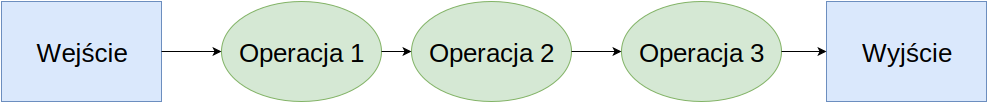
\includegraphics[width=1\textwidth]{img/batch}
	\caption{Procesowanie wsadowe}
  \label{fig:BatchProcessing}
\end{figure}
Takie podejście jest bardzo wygodne z punktu widzenia użytkowania,
po zdefiniowaniu wszystkich operacji oraz dostarczeniu danych wejściowych
proces nie wymaga żadnych dodatkowych czynności ze strony użytkownika.
Dodatkowo z uwagi na swój jednorazowy charakter wiadomo także czy operacje się udały czy nie.

Najpowszechniejszą architekturą wykorzystywaną w przetwarzaniu wsadowym jest \textit{Map Reduce}.
Schemat rozwiązania przedstawiono na rysunku \ref{fig:MapReduce}.
\begin{figure}[htbp]
\centering
	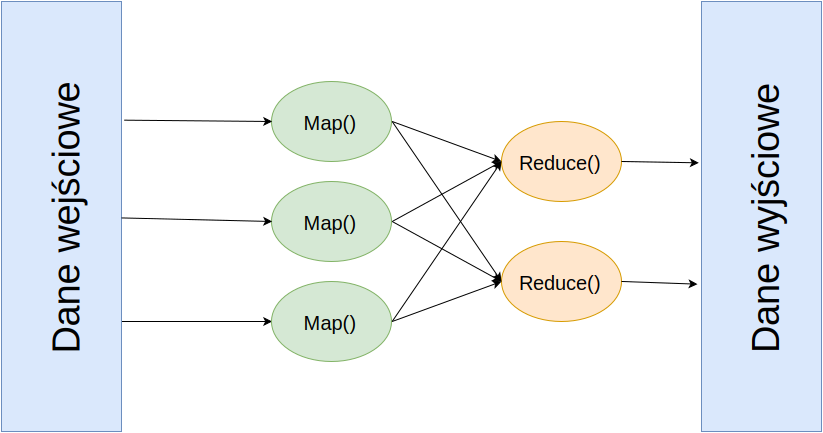
\includegraphics[width=0.9\textwidth]{img/mr}
	\caption{Model architektury rozwiązania \textit{Map Reduce}}
  \label{fig:MapReduce}
\end{figure}
Dane dzielone są na wiele,
niezależnych od siebie zbiorów,
na których wykonywane są różnego rodzaju przekształcenia,
operacje (faza \textbf{Map}).
Po wykonaniu wszystkich obliczeń następuje etap agregowania (faza \textbf{Reduce}) otrzymanych wyników.
Zyski z takiego podejścia najlepiej są widoczne w środowisku rozproszonym (wiele maszyn, procesów i wątków),
gdzie dzięki dekompozycji zadania wzrastają możliwości skalowania.

% TODO:
% Przykłady
% koszyk w supermarkecie

\subsection{Przetwarzanie strumieniowe}

Wymagania użytkowników co do czasu otrzymania wyniku
oraz pewna klasa problemów charakteryzujących się:
\begin{enumerate}
	\item dużą szybkością napływania danych -- dane z czujników, sensorów, etc.,
	\item małymi opóźnieniami (\textit{latancy}) podczas procesowani -- wykrywanie oszustw (\textit{fraud detection}),
\end{enumerate}
powodują,
że metody przetwarzania wsadowego nie znajdują zastosowania.
Podejście strumieniowe polega na analizie danych bezpośrednio po ich pojawieniu się.
Nie jest istotny sposób w jaki dane się pojawiają,
ale fakt,
że są procesowane natychmiast po pojawieniu się.
Mechanizmy analizy strumieniowej można podzielić na 2 typy z uwagi na sposób przetwarzania:
\begin{itemize}
	\item \textbf{Niezależne}.
	Każdy nowy element (zdarzenie) jest przetwarzany pojedynczo i niezależnie od innych.
	Po wykonaniu operacji przekazywany jest do nowego strumienia bądź umieszczany w strumieniu wyjściowym.
	\item \textbf{Buforowane}.
	Elementy napływające ze strumienia przetrzymywane są przez zdefiniowany okres czasu
	bądź czekają na zebranie wystarczającej liczby elementów.
	Po spełnieniu wymaganego warunku są procesowane
	i tak jak w przypadku procesowania niezależnego	przekazywanie dalej albo na wyjście.
\end{itemize}

% TODO:
% Przykład

\section{Platformy streamingowe}

Obecnie na rynku dostępnych jest wiele rozwiązań oferujących analizę strumieniową.
Poprzez rozwiązania komercyjne od gigantów jak Microsoft, Google, Amazon,
po typu open-source,
takie jak Apache Storm, Apache Spark czy Apache Flink.
W ramach przygotowań przed rozpoczęciem prac została dokonana analiza
możliwości i przydatności 3 platform:
\begin{enumerate}
	\item Esper,
	\item Apache Spark,
	\item Apache Storm.
\end{enumerate}
Przy wyborze porównywanych rozwiązań wzięto pod uwagę
łatwość korzystania,
dojrzałość rynkową
oraz aktywną społeczność.

\subsection{Esper}
Esper firmy EsperTech Inc. jest silnikiem umożliwiającym złożoną analizę zdarzeń
(\textit{Complex Event Processing, CEP}).
możliwym do osadzenia w dowolnej aplikacji Java lub .Net.
Esper dzięki swojemu bardzo ekspresywnemu językowi umożliwia na swobodne manipulowanie strumieniami danych.

Język Esper to specjalnie przygotowany język domenowy (\textit{domain specific language, DSL}) do obsługi zdarzeń.
Język ma formę zapytań (kwerend) i został oparty na standardzie \textit{SQL}.

\begin{lstlisting}[captionpos=b, caption=Przykładowe zapytanie w języku Esper]
  select * from StockTickEvent(symbol='IBM').win:length(100)
\end{lstlisting}

Niewątpliwie jedną z głównych zalet Espera jest jego prostota instalacji.
Wystarczy dołączyć bibliotekę,
która jest w formie pojedynczego pliku \textit{jar}
do aplikacji i rozwiązanie jest gotowe do użytku.
Kolejną zaletą jest język dający szerokie pole do działania.
Dzięki oparciu go o klasyczny \textit{SQL} język ten jest zrozumiały dla osób dopiero rozpoczynających naukę,
jak i dla osób bez podstaw informatycznych.
Dostępne funkcje to:
filtrowanie wyników
\begin{lstlisting}
  select * from
    StockTickEvent
  where symbol='IBM'
\end{lstlisting}
funkcje agregujace
\begin{lstlisting}
  select symbol, avg(value) as value from
    StockTickEvent
  group by symbol
\end{lstlisting}
funkcje grupujące (\textit{window functions})
\begin{lstlisting}
  select * from
    StockTickEvent.win:length(100)
\end{lstlisting}
łączenie strumieni
\begin{lstlisting}
  select * from
    TickEvent.std:unique(symbol) as t,
    NewsEvent.std:unique(symbol) as n
  where t.symbol = n.symbol
\end{lstlisting}
tworzenie nowych strumieni
\begin{lstlisting}
  insert into IbmStockTickEvent
  select * from
    StockTickEvent
  where symbol='IBM'
\end{lstlisting}

Niestety to co okazało się zaletą Espera czyli prostota instalacji
jest także jego wadą.
Esper nie ma żadnych wbudowanych mechanizmów ułatwiających skalowanie,
tj. jest tak samo skalowalny jak aplikacja w której został osadzony.

Esper nie daje żadnych gwarancji przetworzenia wiadomości.
Przetwarzane wiadomości znajdują się wyłącznie w pamięci komputera (\textit{in-memory}),
nie są w żaden sposób nigdzie zapisywane,
tak więc w razie awarii węzła tracone są bezpowrotnie.

\subsection{Apache Spark}
Apache Spark jest narzędziem mającym swoje początki na uniwersytecie Berkley.
Jest to ogólnego przeznaczenia framework do zadań obliczeniowych,
charakteryzujący się dobrymi właściwościa skalowania.
Wykorzystywany jest z powodzeniem w operacjach związanych z:
\begin{itemize}
  \item uczeniem maszynowym,
  \item klasteryzacją dużej ilości danych,
  \item analizą strumieniową.
\end{itemize}

% napisany w scali

Jednym z ciekawych elementów tego frameworka
jest możliwość korzystania z jego API w innych językach niż tylko z rodziny jvm (\textit{Java Virtual Machine}).
Oprócz scali czy javy dostepne są:
\begin{itemize}
  \item python
  \item R
\end{itemize}

% moduly
% jak dziala
% zalety

\subsection{Apache Storm}
Apache Storm jest frameworkiem umożliwiającym strumieniowe przetwarzanie danych w czasie rzeczywistym.
Charakteryzuje się przy tym:
\begin{itemize}
  \item skalowalnością,
  \item odpornością na awarię,
  \item niezawodnością.
\end{itemize}
Stworzony został przez inżynierów z firmy
Backtype (Marz, 2014),
a po jej przejęciu, rozwijany przez inżynierów Twittera.
Obecnie projekt został otwarty publicznie dla społeczności \textit{open-source}
i jest nadzorowany przez fundację Apache.

\subsubsection*{Elementy składowe Storm}
\label{subs:StormElemets}
W przypadku Storma reprezentacja zadania nazywana jest topologią (\textit{topology}).
Jest to acykliczny graf skierowany (rys. \ref{fig:StormTopology}).
Elementami grafu są strumienie danych,
elementy tworzące strumień (\textit{spouts})
i elementy operacyjne (\textit{bolts}).
Topologie Storm koncepcyjnie zbliżone są do zadań z przetwarzania wsadowego.
Różnią się tym,
że gdy zadania wsadowe mają jasno określone momenty startu i końca,
to topologię działają nieprzerwanie, do czasu gdy zostaną jawnie zatrzymane.
\begin{figure}[htbp]
  \centering
  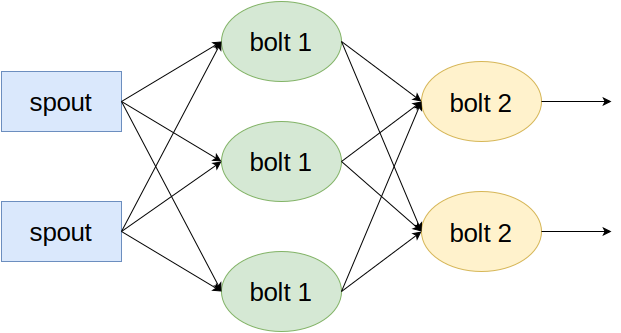
\includegraphics[width=0.9\textwidth]{img/storm}
  \caption{Topologia Storm}
  \label{fig:StormTopology}
\end{figure}

\subsubsection*{Strumienie}
Podstawową strukturą danych w systemach Storm jest krotka (\textit{tuple}).
Krotka jest zbiorem par klucz-wartość przepływających pomiędzy elementami topologi.
Krotka w połączeniu z innymi krotkami tworzy strumień danych.
\subsubsection*{Spouts}
\textit{Spouts} reprezentują punkty wejścia krotek do topologi Storm.
Strumienie mają właśnie swój początek w elementach typu \textit{spouts}.
Przykładowo mogą to być:
\begin{itemize}
  \item dane z sensorów, czujników,
  \item informacje z serwisów społecznościowych,
  \item logi aplikacyjne.
\end{itemize}
\subsubsection*{Bolts}
\textit{Bolts} są elementami w topologiach,
w których wykonywana jest właściwa praca na danych.
Mogą przyjmować na wejście dowolną liczbę strumieni,
przeprocesować je
i jeśli zajdzie taka potrzeba stworzyć nowe strumienie.
\textit{Bolts} mogą podłączać się do strumieni generowanych przez \textit{spouts},
jak i do innych \textit{bolts}.
Dzięki temu można tworzyć skomplikowane struktury przepływów strumieni danych.
Typowymi zastosowaniami \textit{bolts} są:
\begin{itemize}
  \item filtrowanie,
  \item preprocesowanie danych (oczyszczanie, standaryzowanie formatów),
  \item operacje biznesowe,
  \item zapisy w bazach danych.
\end{itemize}

\subsubsection*{Mechanizmy procesowania rozproszonego}
Storm od początku projektowany był z myślą o procesowaniu rozproszonym,
pozwalającym na łatwe skalowanie horyzontalne.
Zadania dzielone są na wiele niezależnych od siebie pod-zadań,
które mogą być uruchamiane równolegle na wielu maszynach na raz.

Elementy ułatwiające realizację wymagań można podzielić na cztery główne grupy.
\begin{enumerate}
  \item Węzły (\textit{nodes}) są pojedynczymi maszynami podłączonymi do klastra Storm,
  na których wykonywane są topologie.
  \item Procesy (\textit{workers}) są fizyczne procesy uruchamiane na węzłach.
  Na jednym węźle może być uruchomionych więcej niż jeden proces.
  \item Wątki (\textit{executors}) są to standardowe wątki uruchomiana wewnątrz procesów.
  \item Zadania (\textit{tasks}) są instancjami obiektów typu \textit{spouts} i \textit{bolts}.
  Operacje są wywoływane przez wątki.
\end{enumerate}
Zależności elementów pomiędzy sobą przedstawiono na rysunku \ref{fig:StormParallel}.
\begin{figure}[htbp]
  \centering
  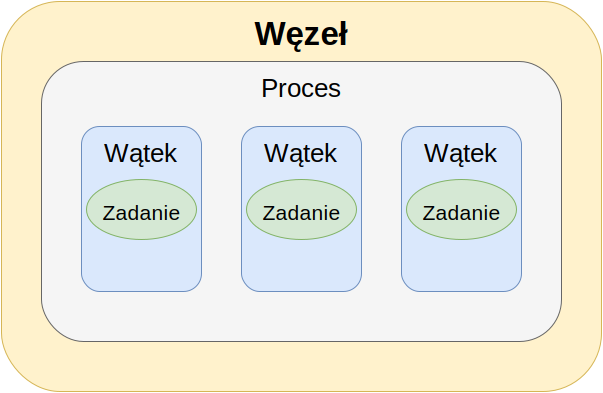
\includegraphics[width=0.8\textwidth]{img/stormElements}
  \caption{Elementy tworzące topologię Storm}
  \label{fig:StormParallel}
\end{figure}

\subsubsection*{Zarządzanie klastrem}
Klaster Storma wykorzystuje klasyczne podejście \textit{master}/\textit{slave}
jednak w trochę innym znaczeniu.
W architekturze typu \textit{master}/\textit{slave} najczęściej jest jeden węzeł nadrzędny (\textit{master}),
który jest wcześniej zapisany w konfiguracji
bądź jest wybierany dynamicznie po starcie.
W przypadku Storma zostało zastosowane drugie podejście.
Klaster Storma (rys. \ref{fig:StormCluster}) składa się z jednego węzła \textit{master} nazywanego \textit{nimbus}
i jednego bądź więcej węzłów pomocniczych nazywanych zarządcami (\textit{supervisors})
Dodatkowo do koordynacji komunikacji pomiędzy nimbusem,
a zarządcami wykorzystywany jest Apache ZooKeeper.
\begin{figure}[htbp]
  \centering
  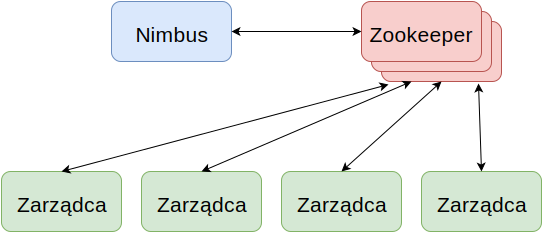
\includegraphics[width=0.8\textwidth]{img/stormCluster}
  \caption{Elementry klastra Storm}
  \label{fig:StormCluster}
\end{figure}

Węzeł \textit{nimbus} jest odpowiedzialny za zarządzanie,
koordynowanie i monitorowania wszystkich topologi pracujących w klastrze.
Dodatkowo zajmuje się także przydziałem zadań dla krotek
oraz pilmowaniem by wszystkie zadania zostały wykonane.
W przypadku awiarii \textit{nimbus} uruchamia ponownie zadanie w innym miejscu klastra.
Węzeł zarządzający odpowiedzialny jest za przydział zadań otrzymanych z \textit{nimbusa}.
Tworzy nowy procesy (\textit{workers}) w ramach węzła,
przydziele do nich zadania.


\section{Podsumowanie}
\begin{table}[h]
  \caption{Porównanie platform}
  \label{stream-summary-table}
  \begin{tabular}{l l l l}
     & Esper & Spark & Storm \\
    \hline
    Analiza strumieniowa w czasie rzeczywistym & tak & nie & tak \\
    Skalowalność & nie & tak & tak \\
    Języki & jvm, .Net & jvm, python, R & jvm \\
  \end{tabular}
\end{table}


\chapter*{Bibliografia}

\begin{references}

\item
Gartner Inc. (2012). \textit{Data management controlling data volume velocity and variety}.
www.blogs.gartner.com/doug-laney/files/2012/01/ad949-3D-Data-Management-Controlling-Data-Volume-Velocity-and-Variety.pdf

\item
Gartner Inc. (2015). \textit{Press release}.
www.gartner.com/newsroom/id/3165317

\item
Marz N. (2014). \textit{History of Apache Storm and lessons learned}.
www.nathanmarz.com/blog/history-of-apache-storm-and-lessons-learned.html

\end{references}


\begin{appendices}
	\chapter{Spis zawartości płyty CD}
	W niniejszym dodatku przedstawiono informacje dotyczące płyty CD dołączonej do pracy.
 	Strukura katalogów wygląda następująco:
	\begin{enumerate}
		\item \textbf{praca dyplomowa} - katalog zawierający plik z pracą dyplomową,
		\item \textbf{latex} - katalog z plikami latex pracy dyplomowej,
		\item \textbf{kody żródłowe} - katalog z kodami źródłowymi skryptów plików, etc. wykorzystanych w pracy,
		\item \textbf{wyniki badań} - katalog z rezultatami badań.
	\end{enumerate}
\end{appendices}

\end{document}
